\documentclass{sig-alternate}
\usepackage{amsmath,amsfonts}
\usepackage{booktabs}
\usepackage{multirow}

\begin{document}

\title{Learning to Assess the Cognitive Capacity of Human Partners}

\numberofauthors{3} 

\author{
%
\alignauthor
Matthew Atkins\\
       \affaddr{Oklahoma State University}\\
       \affaddr{Robotics Cognition Laboratory}\\
       \affaddr{Stillwater, Oklahoma 74078}\\
       \email{matthew.atkins@okstate.edu}
% 2nd. author
\alignauthor
S. M. Al Mahi\\
       \affaddr{Oklahoma State University}\\
       \affaddr{Robotics Cognition Laboratory}\\
       \affaddr{Stillwater, Oklahoma 74078}\\
       \email{smahi@okstate.edu}
% 3rd. author
\alignauthor Christopher Crick\\
       \affaddr{Oklahoma State University}\\
       \affaddr{Robotics Cognition Laboratory}\\
       \affaddr{Stillwater, Oklahoma 74078}\\
       \email{chriscrick@cs.okstate.edu}
}

\maketitle
\begin{abstract} 
We demonstrate that a robot is capable of learning to recognize the
behavioral indicators that a complex, rapidly-evolving task has exceeded
the cognitive capacity of a human partner and make an informed decision
based upon this assessment. The robot is trained to associate human
directions with task quality for a well-understood task, in this case, the
navigation of a maze. The robot may then apply this learned model to a
different problem while still being able to evaluate a human operator's
cognitive load. Even without the ability to understand the end goal of this
new task, the robot can use the indicators learned previously to estimate
the cognitive limits of an increasingly frazzled human partner.. Perhaps
even more importantly, the robot may then make an informed decision
based on this assessment, switching to an autonomous operation mode for
example, in an attempt to reduce operator demand.
\end{abstract}

%\category{I.2.9}{Robotics}{Human Assistance}{Multiple Robots}

%\terms{Cognitive Limitation, Trust, Mobile Robot}

\keywords{User modeling and awareness, teamwork and group dynamics,
  robot behavior design, quantitative field study, learning about the
  environment}

\section{Introduction}
One of the most challenging obstacles facing human-robot teams is the
inherent communication barrier between the two. Human operators, at
least once they have received training, have some notion concerning
the capacities of their mechanized partners, but the ability of robots
to assess the limitations of humans has not received adequate
attention. Research in this area often focuses on attempting to
observe human behavior and predict what action or actions to perform
in the future; this renders such systems incapable of making
instantaneous or reactive decisions. In contrast, systems which are
capable of making split-second decisions, such as the lane drift
detection found in some high-end cars, make no inference concerning
the user's abilities or frame of mind; they are reacting to a
well understood world state without consulting their human
partners. This is not true interaction; the robot is learning to work
\textit{around} the user instead of with them. Human assistance
should enable complex multi-robot tasks in situations where the robots
themselves are unable to assess their environment fully, but this lays a
heavy burden on the operator in a dynamic, dangerous, rapidly-changing
environment with many cognitive demands. Human
operators and robots each have complementary capabilities and
limitations; that both groups have the ability to know the limits of the other is crucial for cooperation and ultimately success. \cite{Malchus:2013:REC:2447556.2447632}.

Our research allows robots to form models of human behavior during
well-understood tasks, and then apply these learned models during
unknown tasks. We show that these models allow the robot to make an
effective determination of the cognitive capacity of a human partner,
even when the robot cannot directly assess the task it is being asked
to perform. This provides the robot with the ability to fall back to safe
autonomous operation mode whenever the task demands begin to
exceed the ability of its human partner. The operator may then assume direct control at their discretion as they are able.

\begin{figure}
\centering
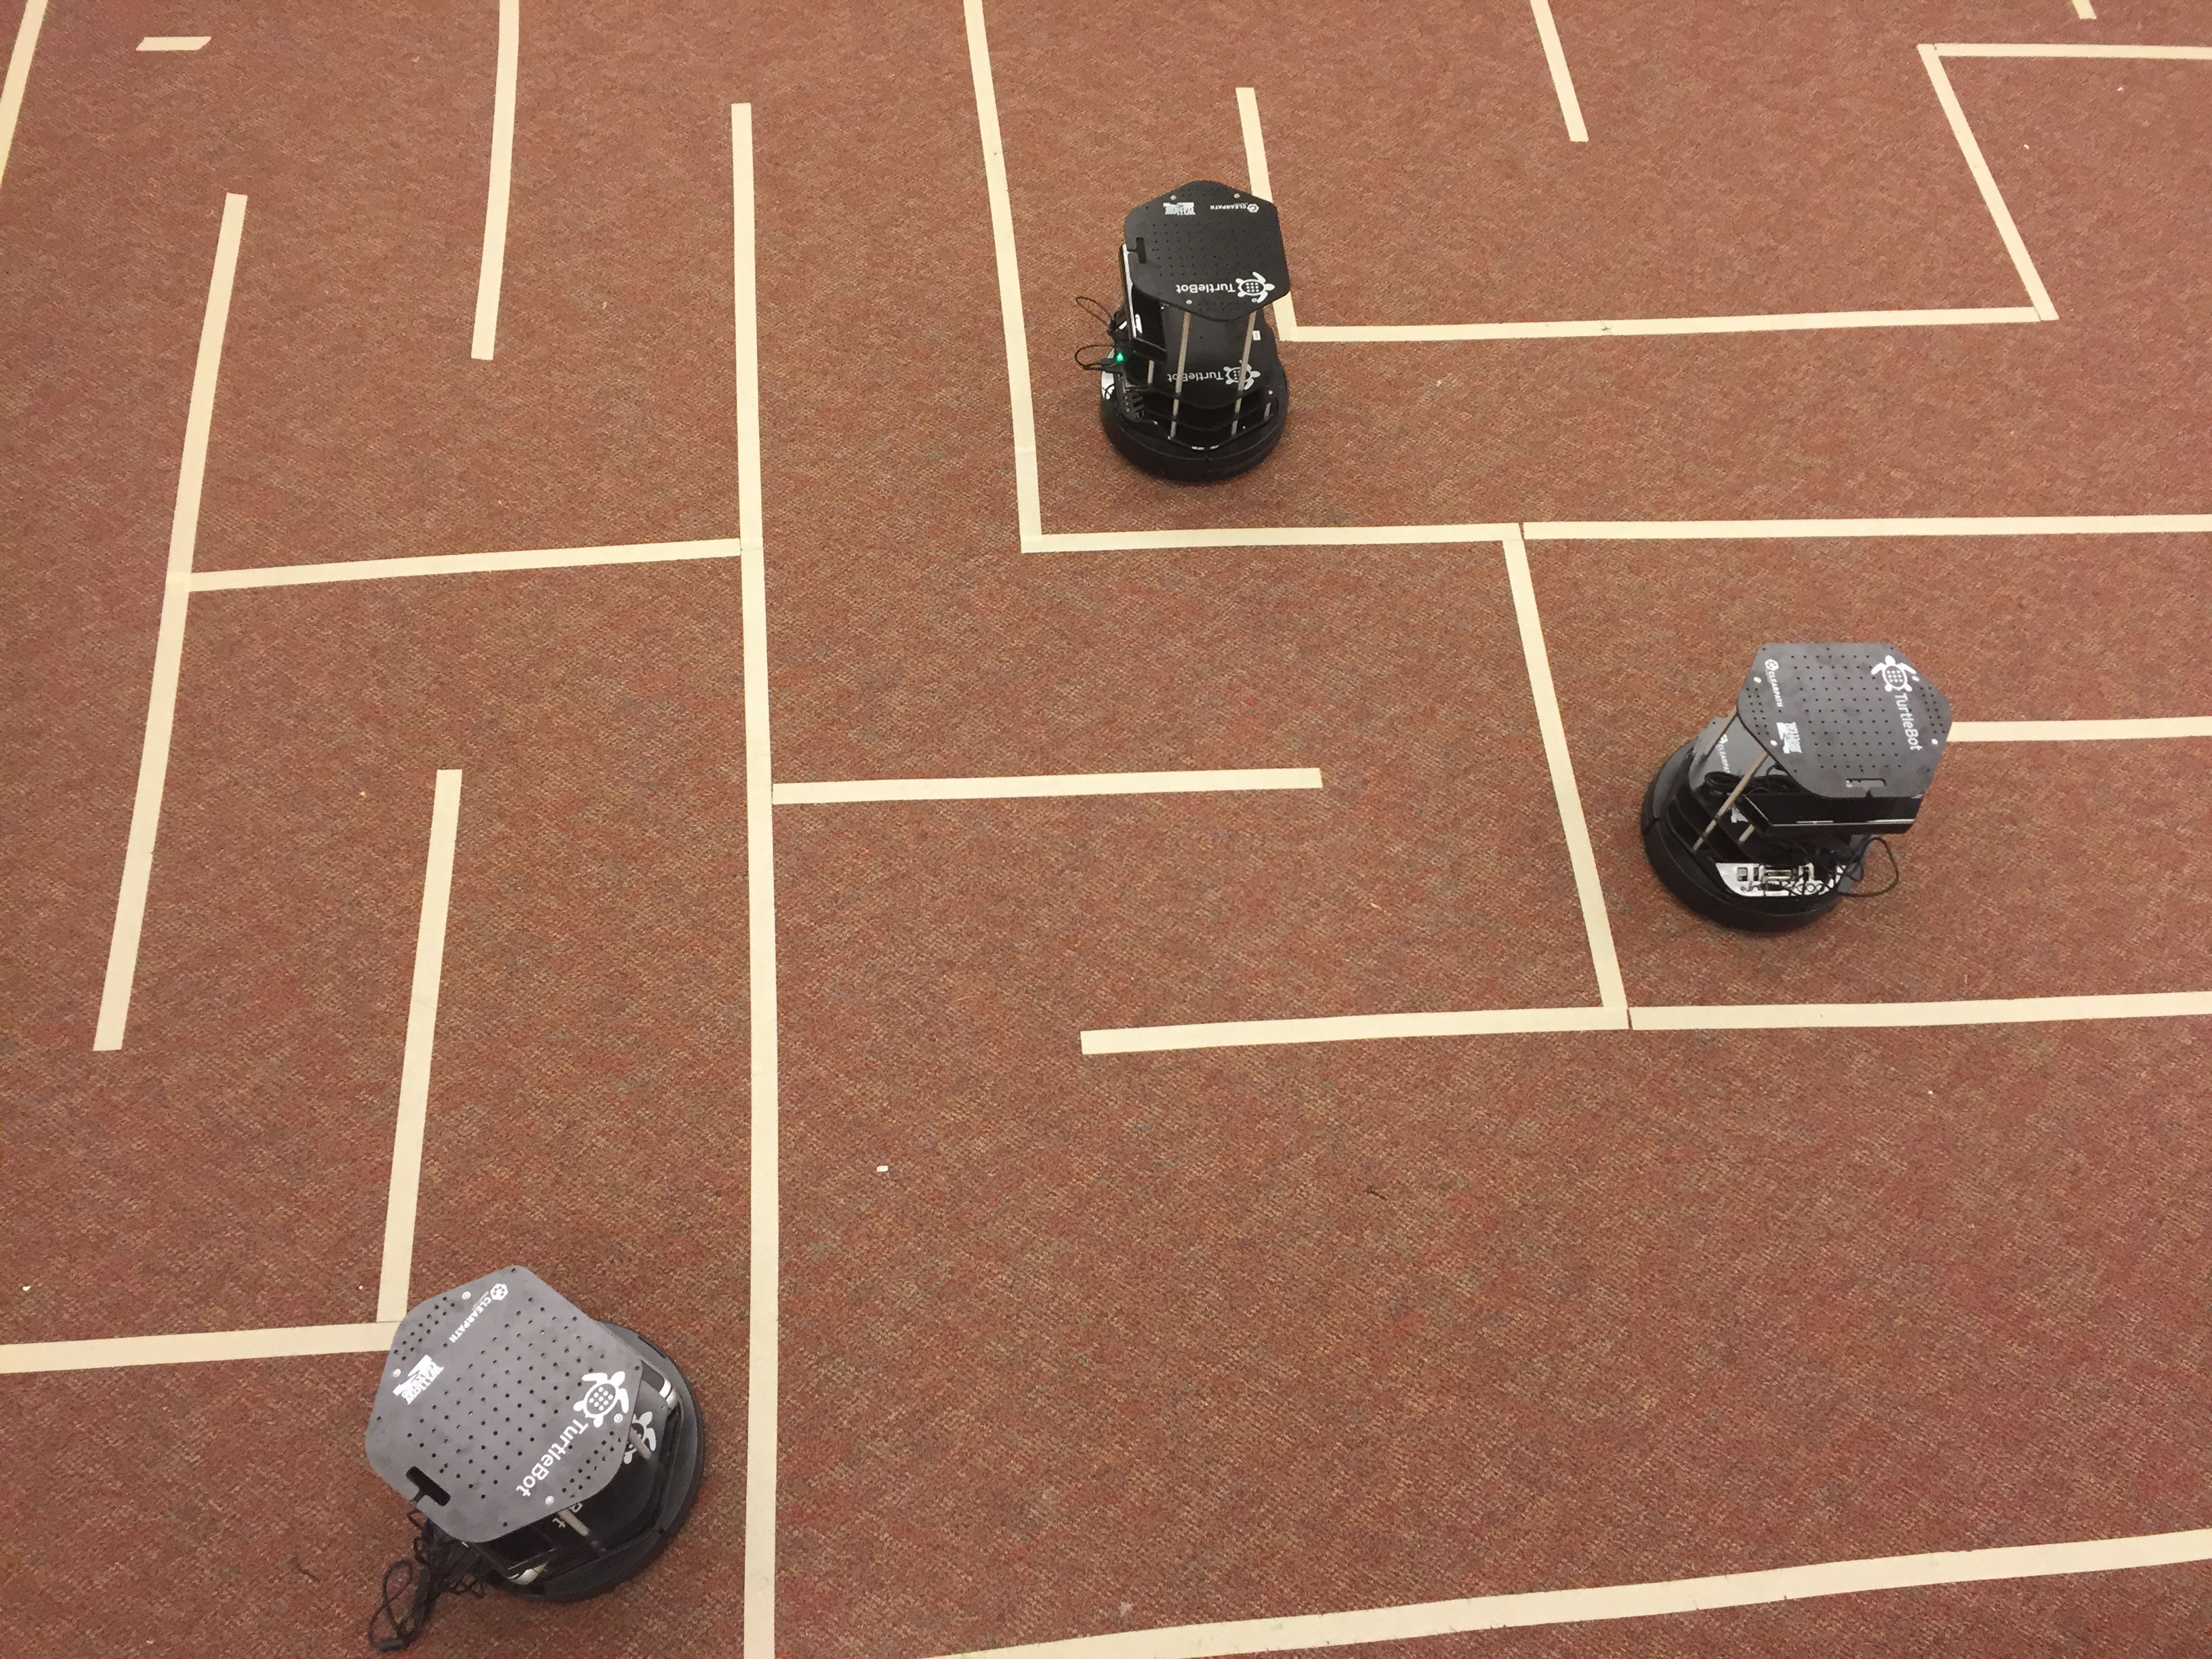
\includegraphics[width=.5\textwidth]{robots-in-maze.jpg}
\caption{Turtlebots navigate a maze while evaluating human task input.}
\label{fig:game_photo}
\end{figure}

Why is this understanding between human and robots so important? As
previously mentioned, both members have advantages and limitations. It
easy to see that a robot with limited sensors and actuators may be unable
to perform a task, owing to a failure to perceive information about its
environment. Merely cramming improved components into a robots does
not guarantee any significant improvement on the robot's ability to
accomplish a task -- a great many tasks require contextual information far
beyond what machines are currently able to muddle out. Thus for the
foreseeable future, many of these complex tasks will require assistance
from human teammates, co-processors if you will. Humans are able to
integrate data, rely on experience to predict the effects of actions on world
states, and produce effective long-term plans far better than any current
robot.

Human assistance with multiple robots has been demonstrated in
different practical situations. For example, they have been used as
customer assistants in shopping malls \cite{zheng2013supervisory,
  Kanda:2009:AGR:1514095.1514127}, where human operators occasionally
assisted robots. Human-robot teams have assisted each other in museum
tour scenarios \cite{thrun1999minerva} and in warehouse inventory
management \cite{wurman2008coordinating}.  Just as robots, regardless
of their hardware capabilities, do not necessarily perform well
without assistance, humans do not always assist robots as efficiently
as they might, despite their superiority in context sensitivity and
general intelligence.  Several issues arise in this regard
\cite{breazeal2004social}, including obvious problems such as noisy
communication between human operators and robots, accidental damage to robot sensors and so on.

In this paper, we focus on one problem which can cause difficulties in
a human-robot team: the cognitive capacity of the human operator.
Humans often find their ability to function effectively challenged,
due to psychological stress, tiredness, or overwhelming task demands.
A robot's ability to participate constructively in a human-robot team
will benefit immensely from understanding and accommodating this
cognitive stress appropriately.  For example, for the pilot of an
unmanned aircraft, cognitive stress can be the difference between life
and death \cite{crandall2005validating}.  If such a robot can detect
the emergence of cognitive stress in its operator, it can increase its
level of autonomy and reduce its demands on the operator's attention.
Hopefully, such a robot would wait safely for a more opportune moment
or decide to engage in a less cognitively challenging task, rather
than continue to follow the direction of a human who is no longer able
to provide appropriate assistance.

In this paper, we have designed robots that learn the correlations
between quantifiable behavior metrics and the cognitive capabilities
of human operators.  We designed a maze game
(Fig. \ref{fig:game_photo}) where multiple robots are given directions
by a single human operator.  At first, the robots' objective was
simply to complete the maze, a task that they were capable of
executing without human assistance using autonomous path planning.
They were therefore able to determine whether the instructions of
their operators were sound or questionable, and associated these
outcomes with measurements of their operator's behavior.  We observed
the output of the learned cognitive stress model in a different task,
this time with the robots engaged in a coin-collecting game inside the
maze.  Although the robots had no knowledge of the rules or objectives
of the coin-collecting game, and had no ability to sense the game's
context, their learned models enabled them to determine the cognitive
stress of their human partner.  In this way, they were able to
evaluate the trustworthiness of the actions they were being asked to
perform.  The cognitive stress discerned by the robot correlates with
the true stress experienced by the human operators, as quantified by
their self-reporting and by expert evaluation.

\section{Related Work}
In this section, we will briefly discuss work related to cognitive
capacity assessment and human operation of multiple robots.  Several
research projects recently have investigated human cognitive capacity
using different approaches.

Effectively navigating a maze game has been demonstrated in literature
\cite{crick2011human}.  This research showed that robots learn more
effectively from human operators if the learning took place in the
context of features that the robot can easily understand.
Counterintuitively, restricting the information available to a human
operator led to better demonstrations and more effective learning.  In
this research, we show that similar metrics can be employed by the
robot for the purpose of learning the cognitive threshold of a human
operator.

Recent work \cite{das2013attention,Hoque:2012:ACH:2157689.2157729}
presented a model for assessing a human's attention level, based on
eye contact and gaze detection towards a robot. Based on the perceived
attention level, the robot could generate an appropriate signal to
obtain the attention of a targeted human.  Attention is an important
component of a human agent's cognitive capacity, but in our work, the
robot learns a general behavior model to identify the operator's
cognitive threshold, rather than relying on the specifics of gaze.

Human-robot interactions can be evaluated using fundamental metrics
\cite{olsen2003metrics}. Such metrics relate to the cognitive capacity
of human operators in obvious ways. For example, task effectiveness
(TE) describes how efficiently robots complete a given task under
human direction.  For example, task effectiveness can be measured
using the speed of the robot. In a navigation experiment, it may be
the time taken by the robot to reach the goal.  It could be defined as
the difference between the time taken with and without human
assistance.  Another important metric is neglect tolerance (NT), which
denotes a robot's level of autonomy. In static indoor environments,
simple robots such as Turtlebots can easily engage in autonomous
navigation. Even in complex environments with dynamic obstacles,
clever algorithms \cite{montemerlo2008junior} can enable such vehicles
to navigate autonomously. Thus although it is a very important metric,
we have focused on mostly TE because we think that that is the metric
which can be exploited more consistently across different problems.
Other potentially useful metrics include robot attention demand (RAD),
free time (FT), fan out (FO) and interaction time.  All of these could
conceivably be included as inputs into a learned model such as ours.

Other efforts \cite{goodrich2003seven, olsen2003metrics} have
presented very similar concepts of metrics for improving the
efficiency of human-robot interaction. These principles include
implicit mode switching among user interfaces, using human operators'
natural cues, directly manipulating the world, manipulating the
relationship between the robot and the world, supporting attention
management and so on. Using similar terminology, other work
\cite{crandall2005validating} discovered how neglect time impacts
important properties of human robot teams. They have shown a relation
between the neglect time and the maximum number of robot that a single
human operator can handle.  We leverage this data to inform our
robots' estimation of a human operator's cognitive capacity.

In another social experiment \cite{zheng2013supervisory}, where
autonomous humanoid robots have been deployed to investigate their
social acceptance, a scheduling algorithm has been used to assist the
human operator.  This experiment developed an algorithm that
prioritizes the assistance provided by a human operator for a
particular robot within a multi-robot team. The robot's task was to
make conversation with interested shopping mall customers and to guide
them to particular shelves corresponding to their needs. The shopping
mall map was already known.  Within critical areas inside the shopping
mall environment, the robot needed assistance from humans, for example
in unsafe locations or areas with glass walls that confused the
robots' sensors.  As there were multiple robots, a single operator
could not assist them all simultaneously.  The operator allocator
algorithm therefore picked the robot most likely to encounter a
critical region for assistance. In this work, the operator was assumed
to be able to assist the robot without considering cognitive
capacity. In contrast, we developed a model that enables the robot to
make this determination and then perform the task accordingly.

A large amount of work
\cite{thomaz2006reinforcement,thomaz2008teachable} has investigated
human operators acting as teachers when interacting with a robot, for
example helping a robot in kitchen environment. The human's
demonstrations contribute to the robot's reward functions, using a
modified reinforcement learning method that is based on the
observation that human guidance is able to consider future reward
along with past reward.  The rich context that a human operator
provides and that robots are very poor at reasoning about for
themselves leads to improvement in the robot's learned behaviors.
This observation only holds, however, as long as the human operator
possesses the cognitive capacity to provide good, informative
demonstrations.  Our work allows robots to make this determination for
themselves.

We have mentioned a number of research results that relate to ours in
many ways.  However, most current work does not explore the fact that,
although humans are much more intelligent than robots, they
nevertheless face significant limitations in their ability to assist
their robot partners.  One aspect of these limitations is that a human
operator is vulnerable to task overload and psychological stress.  Our
work focuses particularly on human behavior in the face of this
cognitive stress.  Although engaging human assistance for the purpose
of task learning is valuable, we argue that such a learning task is
more effective if the robot simultaneously has the tools to evaluate
the trustworthiness of the human's direction.

\section{Technical Details}
\subsection{Problem statement}
Without loss of generality, take $H=[h_1,h_2,\cdots,h_m]$ to be a
vector of ecologically valid measurements of human behavior relevant to
the problem space.  Assume a task for which a robot participant can
independently calculate $s$, a scalar metric of success, which is a
function of a vector of measurable environmental features
$E=[e_1,e_2,\cdots,e_n]$.  Thus, $s = f(E)$, where $f$ is a
task-specific function known to the robot.  Using $f$ and calculating
$s$, a robot can build its own supervised training set for a learning
task, where the human input $H$ is associated with $s$ through a
learned function $g$.  Thus, the robot learns to associate the human
behavioral metrics $H$ with task success $s$ within a known task, so
the output of $g$ is a learned \emph{estimate} of the true success
($\hat{s}=g(H)$).  Now, assign the robot a task which requires human
input for success, i.e., the robot has no access to an analogue to $f$
or $s$ in this new task.  However, it can still measure the components
of $H$, and it has access to its learned model $g$.  We show that
computing $\hat{s}=g(H)$ in this new environment allows the robot to
estimate not the task success (about which it has no information), but
the cognitive load on its human partner and an estimate of the quality
of the human's direction.
\subsection{Experimental design}
In keeping with the problem statement, experiments were carried out in
two parts: the Maze Game and the Coin Game experiments. In the first
phase, the robot collected the data needed to build a model $g$ for
evaluating the trustworthiness of user input $H$. The robot is able to
do this for the first phase because in the case of the Maze Game it
has access to $f$ and $E$ and can calculate $s$.  It understands the
problem sufficiently to make such judgments; the robot requires no
human aid to solve this problem.

%\begin{figure}
%\centering 
%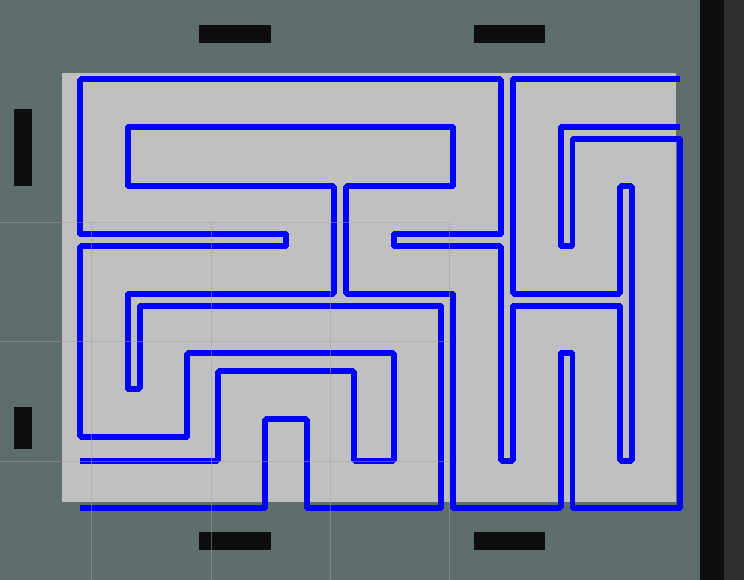
\includegraphics[width=.5\textwidth]{rviz_maze.png} 
%\caption{Representation of the path through the maze in RViz.}
%\label{fig:rviz_map}
%\end{figure}

\begin{figure}
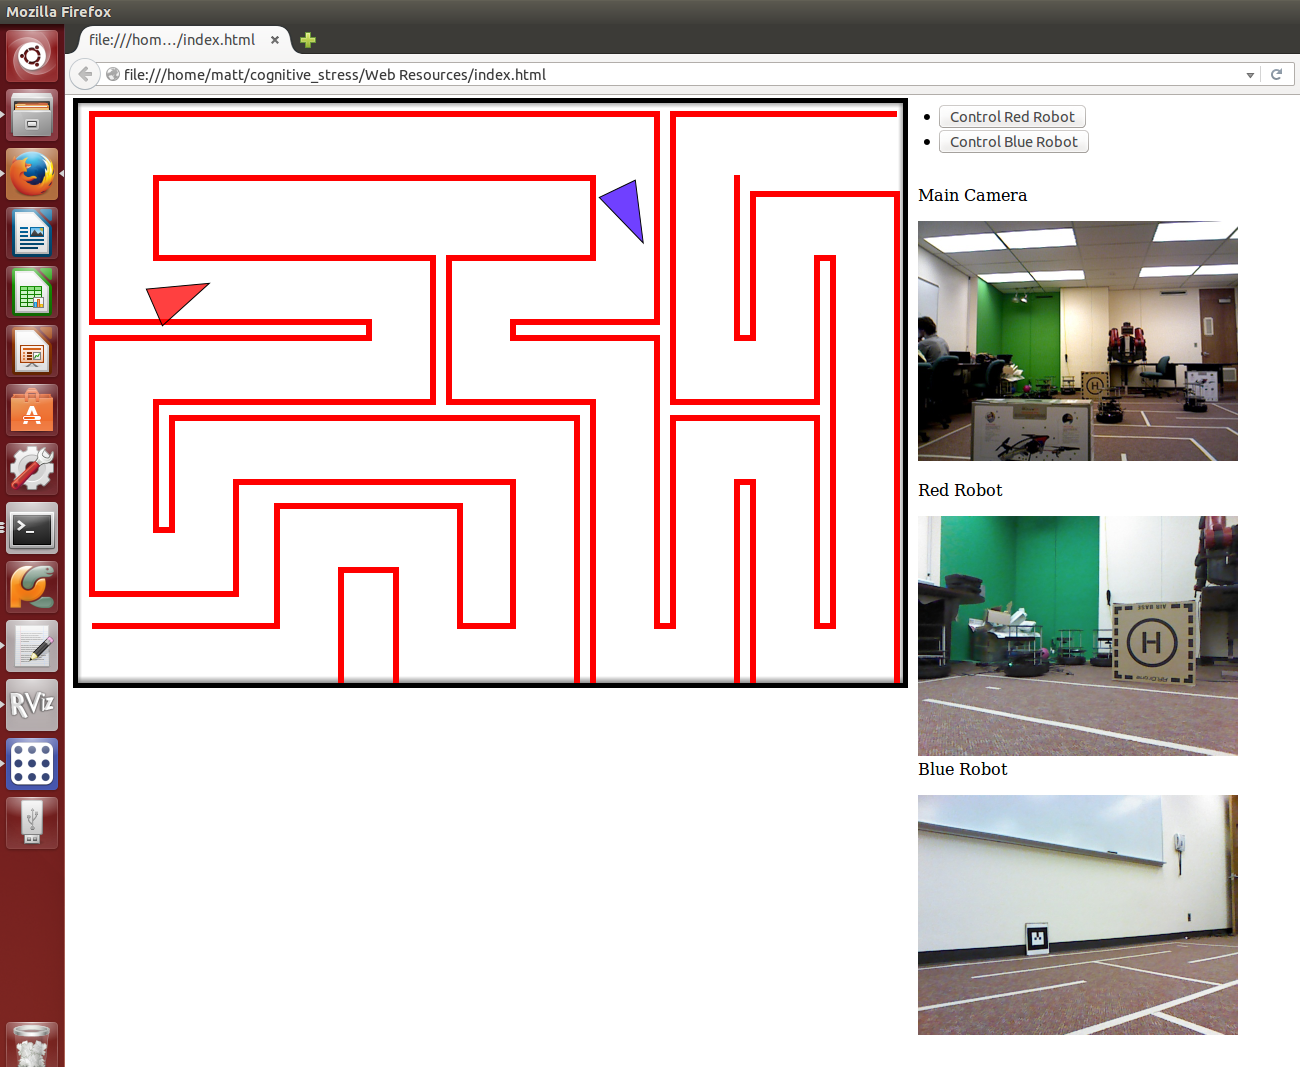
\includegraphics[width=.5\textwidth]{web-controller.png}
\caption{The Rosbridge Web Interface.}
\label{fig:web_interface_img}
\end{figure}

In the subsequent Coin Game, the robot is placed in a different
scenario, one in which it had no access to success measures or even
rules; beyond the fact that it was moving in a similar environment to
the Maze Game, it is wholly reliant on human direction to succeed in
the task.  Even so, with no independent means of measuring task
success, it can still calculate $\hat{s}=g(H)$, and can therefore
evaluate the quality of instruction, and hence the cognitive capacity,
of its human partner.

Communication between operators and robots was achieved using the
Robot Operating System (ROS)\cite{quigley2009ros}.  Users sent
navigation goals to the robots by using a web interface developed for
the project, which allowed the experiment to be conducted remotely
(Fig~\ref{fig:web_interface_img}).

\section{Maze Game and Training}
  
%\begin{figure}
%\centering
%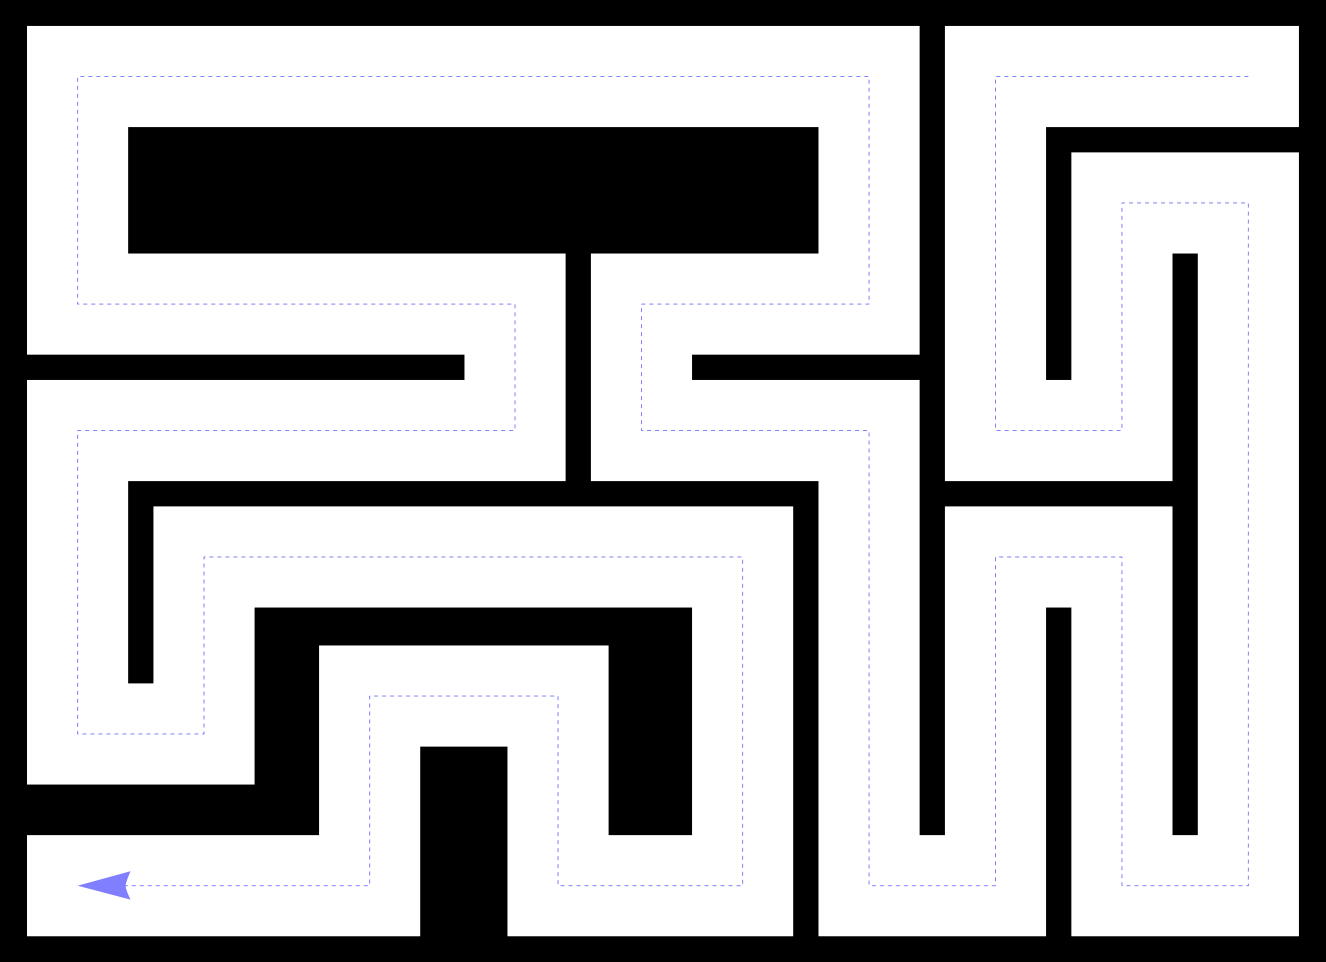
\includegraphics[width=.5\textwidth]{maze-representation.png}
%\caption{Map of the maze.  Arrow indicates path direction.}
%\label{fig:maze_with_path}
%\end{figure}

\begin{figure}
\centering 
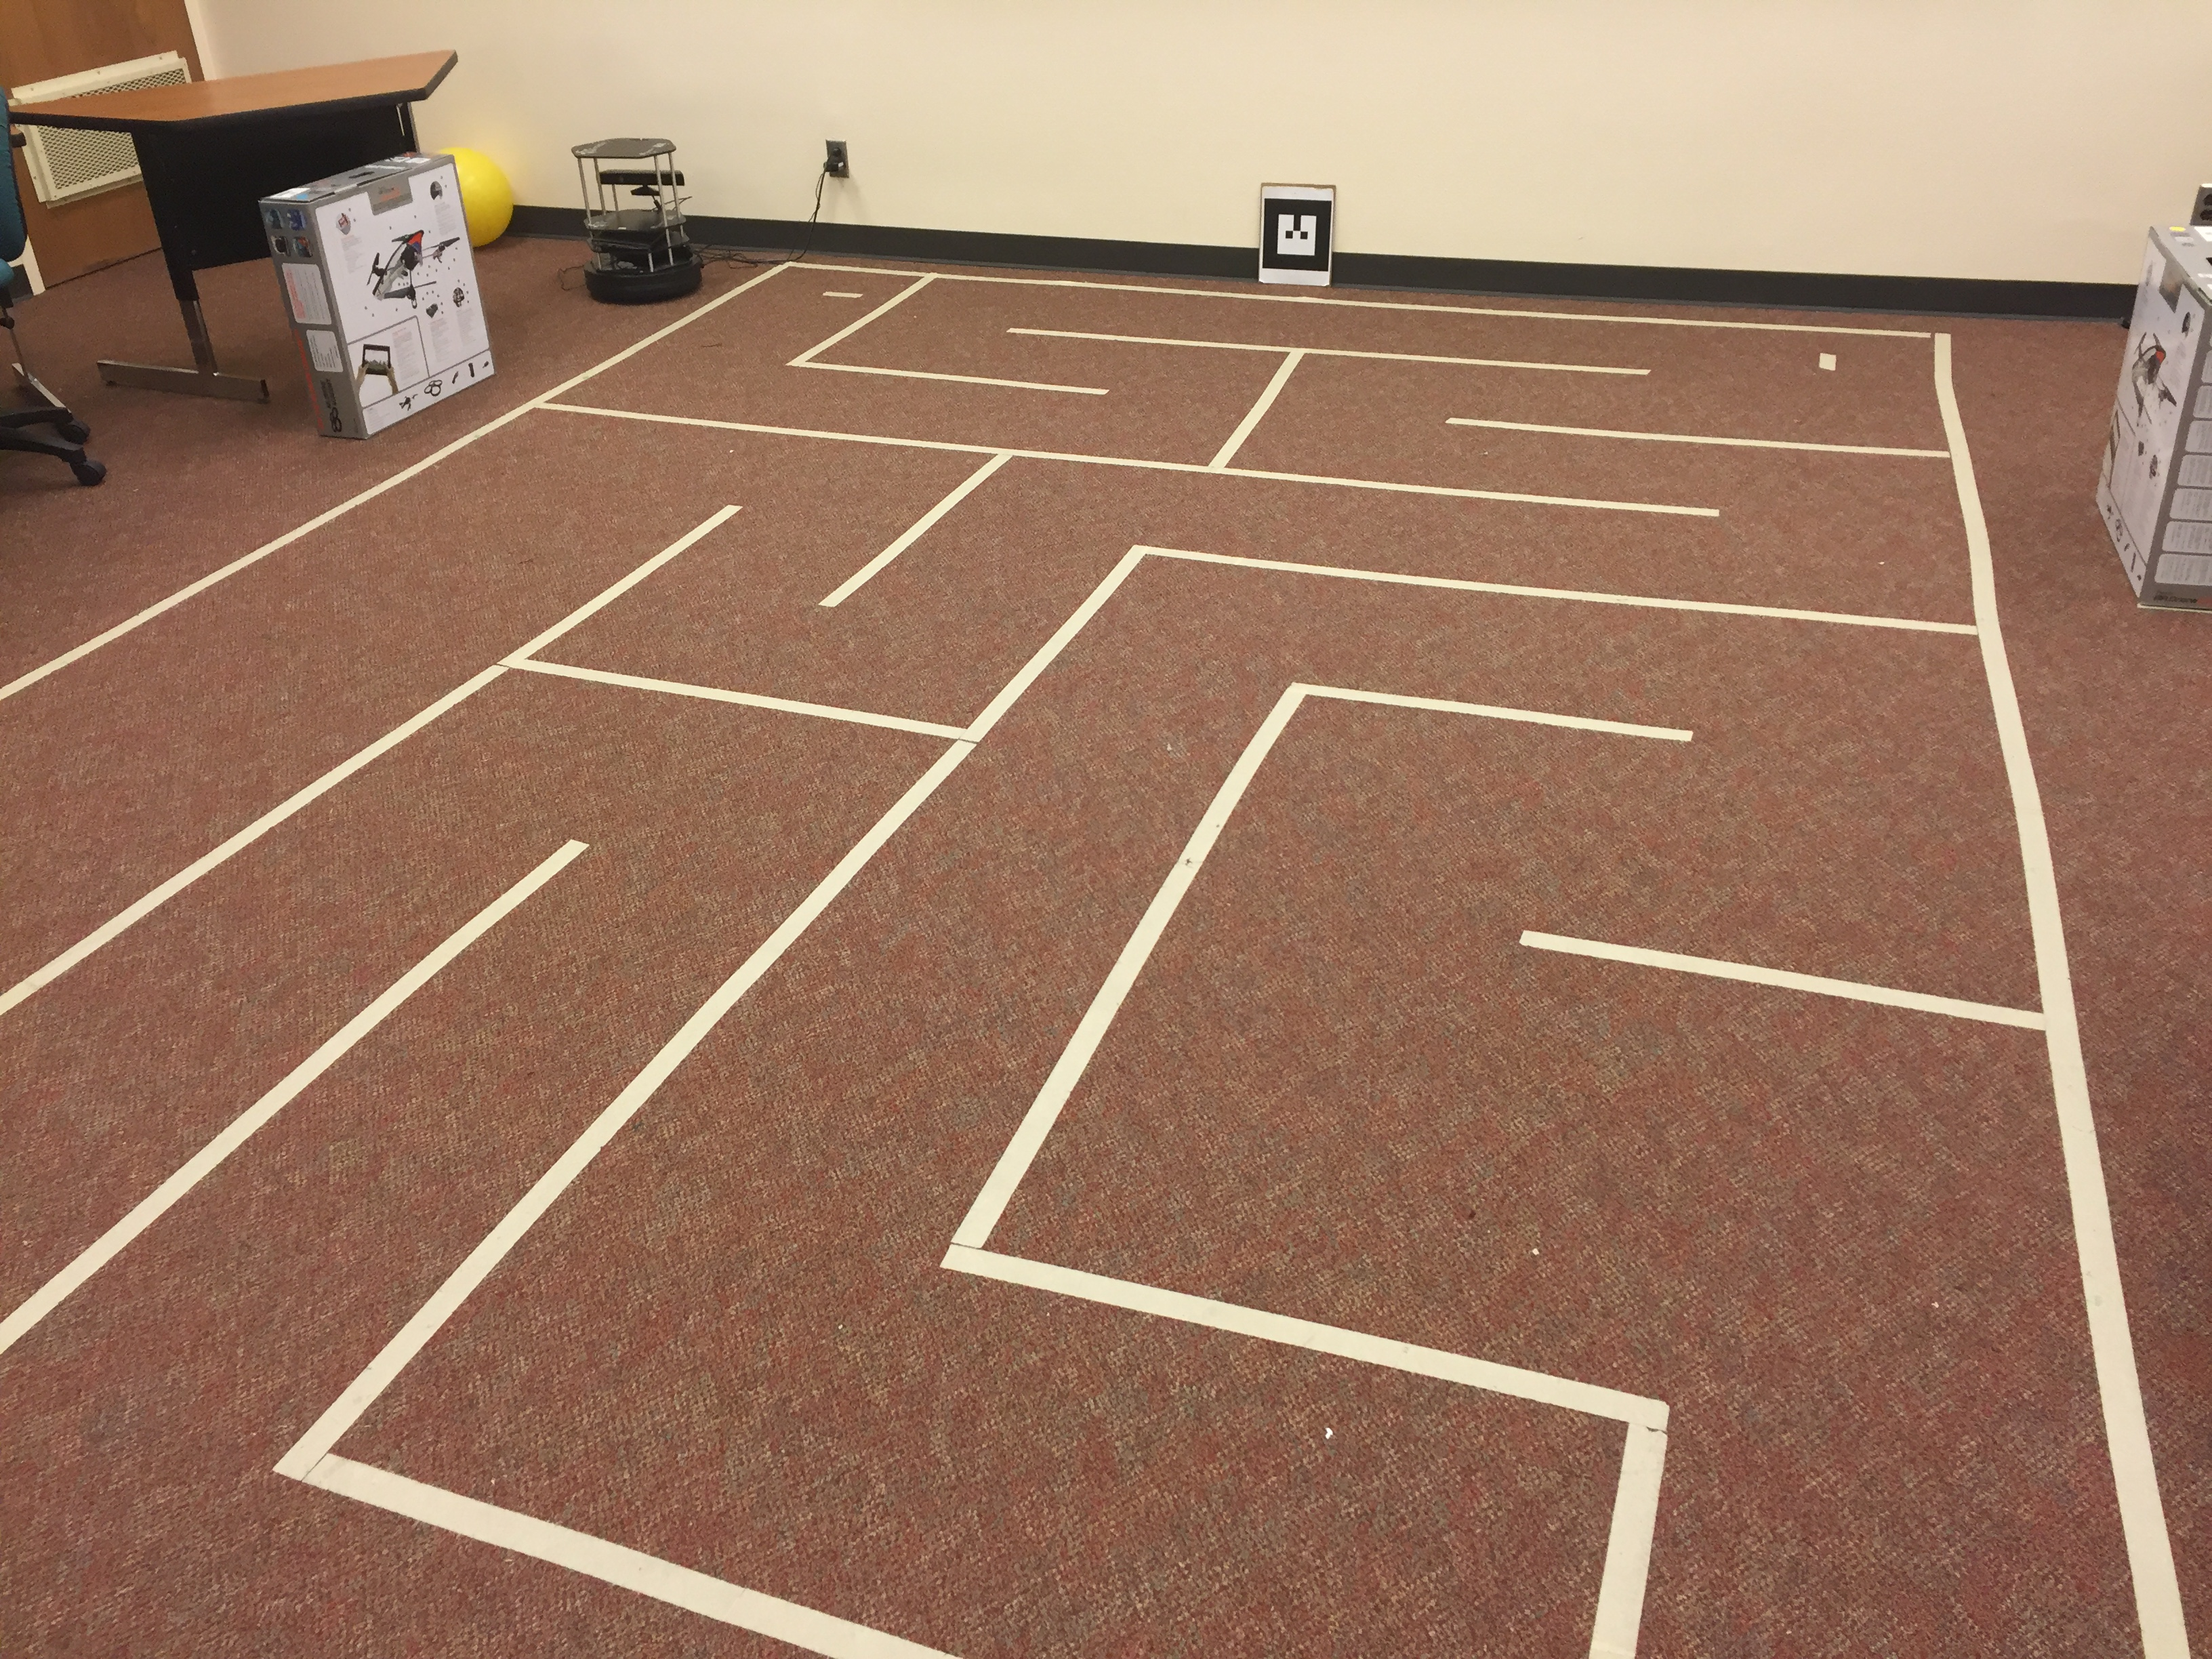
\includegraphics[width=.5\textwidth]{tape_map.jpg} 
\caption{The final map laid out on the lab floor.}
\label{fig:map_floor_img}
\end{figure}

As previously mentioned, the first step of our experimental design was
to identify a task simple enough for the robot to complete unaided,
yet complex enough to potentially benefit from human input. The
problem also need to be readily scalable to include additional
robots. This led us to select autonomous navigation through a maze
using Adaptive Monte Carlo Localization (AMCL). The maze consisted of
a single path with multiple \text{90${}^{\circ}$} turns.  The final
design, seen in Fig~\ref{fig:map_floor_img}, consists of 32 waypoints
and measures $4.63m$ by $3.2m$. It is important to note that the maze
traced out on the floor serves only as a convenience for human
operators and does not serve as a navigation guide for the robot. In
fact, the robot does not treat the walls of the maze as physical
obstacles, and will happily pass through them if instructed to do so.

In the Maze Game, the robot is able to evaluate the success of the
directions it is given by its human operator.  This is a function of a
vector of environmental measurements $E = [e_0, e_1, e_2]$, which in
this particular context have been defined as follows:

\begin{itemize}
\item $e_0$ is the \emph{disparity} term, the distance between the
  navigation directions provided by a human and the route that the
  robot would have planned for itself,
\item $e_1$ is the \emph{collision} term, which penalizes collisions
  with walls, and
\item $e_2$ is the \emph{time delay} term, the amount of time taken
  for the human to guide the robot through the maze, compared with the
  robot's estimate of the time it would have taken under its own power.
\end{itemize}

The computation of $s = f(E)$ to obtain a success metric is
straightforward:

\begin{equation}
s = \frac{1}{Z}\sum_{i=0}^{|E|} e_i
\end{equation}

where $Z$ is a normalization constant.

%  We then define a decision function $\delta$ based on $s$.  This is intended to indicate whether the provided human assistance is qualitatively above or below that person's useful cognitive threshold $\theta$:

%\[
%\delta(i) = 
%\begin{cases}
%True, & \text{if } s\le \theta\\
%False, & Otherwise\\
%\end{cases}
%\]

By computing this value $s$, the robot can label its own data in order
to train a supervised learning algorithm which will relate the success
of a human-directed task (and, presumably, the cognitive capacity of
the human partner) with a set of measured behaviors $H$.

$H = [h_0, h_1, h_2]$ is a set of human behavioral metrics which are
ecologically valid for a navigation direction task.  For this
particular experiment, these are the following:

\begin{itemize}
\item $h_0$ is the \emph{decision interval} term, which measures the
  time elapsed between the robot reaching a navigation goal and the
  human providing a new one,
\item $h_1$ is the \emph{error correction} term, which measures the
  tendency of a human operator to provide a navigation goal and then
  subsequently provide another before the task is complete, and
\item $h_2$ is the \emph{franticness} term, which characterizes erratic behavior for the control inputs.
\end{itemize}

These features were chosen because they are contextually valid for a navigation problem, while remaining general enough to not be tied to our a specific instance. It is worth noting that there is no reason to
assume that the features selected are  uniquely suited as members of $H$.
Appropriate features for inclusion in $H$ should be easy to identify
in a wide variety of tasks.

\subsection{Maze Game and Training Results}
Now we will show that the robot is able to learn the model $\hat{s} =
g(H)$, and that it reflects the cognitive capacity of humans
correctly, based on the described metrics.  Fifteen test subjects
performed runs of the maze game, resulting in approximately $1000$
data points used for training.

%\begin{figure}
%\centering
%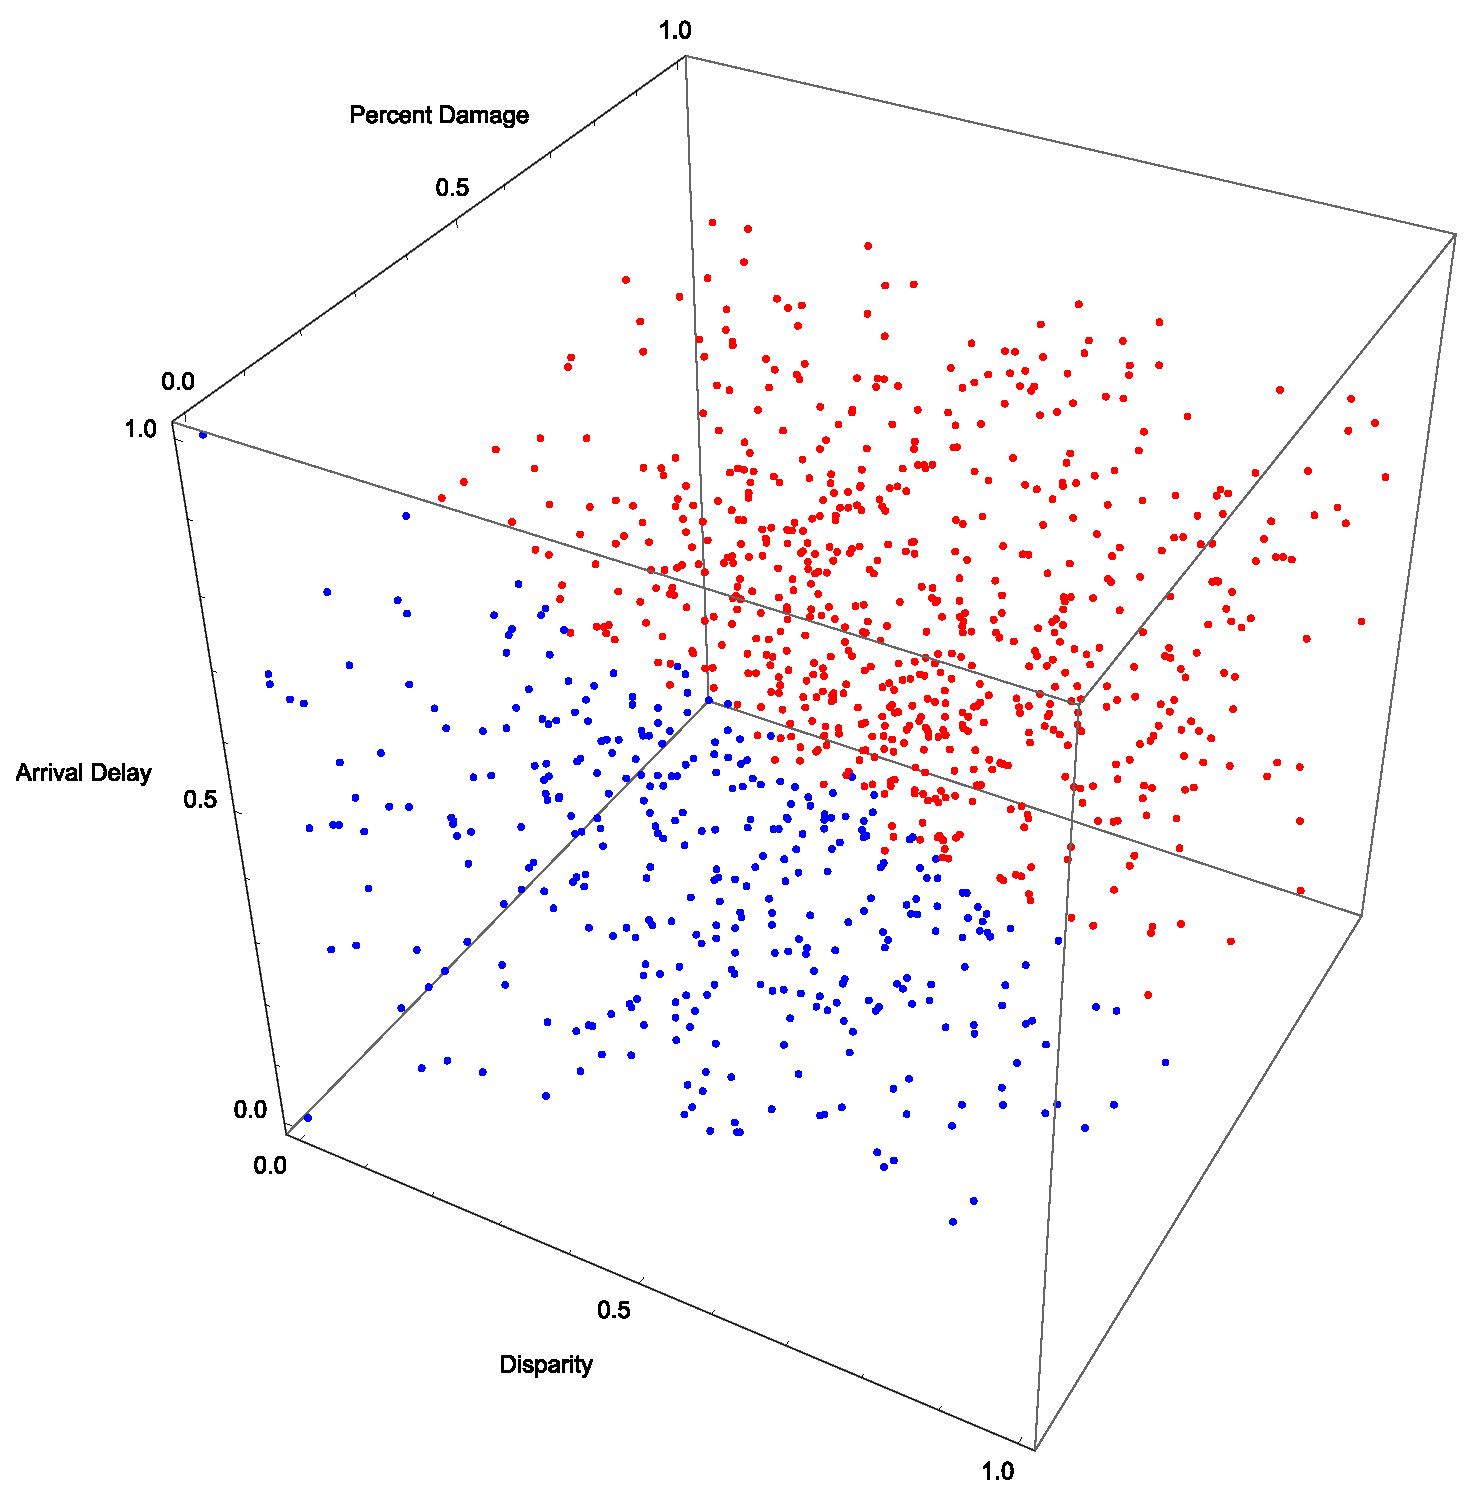
\includegraphics[width=.5\textwidth]{4d-plot.eps}
%\caption{Disparity, Collision, Time Delay vs. Task Success.  The robot
%  has adjudicated red dots as indicating human behavior at or beyond a
%  useful cognitive threshold, and blue dots as trustworthy.}
%\label{fig:data_maze_game}
%\end{figure}

%Fig.~\ref{fig:data_maze_game} shows a four-dimensional scatter plot
%that shows the robot's judgment of human cognitive capacity respect to
%the humans' behavioral metrics.
Because the robot understands the maze game and the details of the
performance metrics, it is able to generate the training data labels
for a supervised model learning task.  We have used the Orange data
mining API\footnote{http://orange.biolab.si} for running the
regression.  The human behavioral metrics $H$ and the robot's
self-generated task success metric $s$ are used to train a Random Forest Regression Learner (RF).RF have been
used to learn enormous classifiers in very complex feature spaces. The maze game regression
operates only in a low-dimensional feature space, so an RF is able to
learn from our experimental data effortlessly, and the approach should
scale to much more complex feature spaces.  The classifier is trained
on $H$ and $s$.  The RF generates an optimized $g(H)$ by performing a
regression on the relationship between $s$ and $H$.
%identifies a regression on the test data by minimizing the
%following function:
%\begin{equation*}
%\begin{array}{ccc}
%\frac{1}{2}w^{T}w + C\sum _{i=1}^N \xi _i \\
%\text{with the following constraints,} \\
%y_{i} = (w^{T}x_{i} + b)\geq 1-\xi_{i} \text{ and } \xi_{i}\geq 0, i=1,...,N
%\end{array}
%\end{equation*}
%Here $C $ and $b $ are constants. $\xi $ denotes the non-separability
%of the input data.

%The classifier was trained using two different methods;
%cross-validation and leave-one-out.  Both of the data sampling methods
%provided good classification accuracy. In the cross-validation method
%we sampled 70\% of the data from the maze game to use as training
%data, which resulted in a 95\% accuracy in the classification on the
%test data sample. In the leave-one-out method, all instances except
%one are selected for training the classifier. After that, the test
%data set is classified using the learned model. All of the instances
%are selected at least once as test data. The total accuracy of the
%classification is calculated by counting the percentage of data that
%has been selected and classified correctly against the total data
%set. This method also resulted in 95\% of the data being correctly
%classified.
%The result of the classifier on the test data using different sampling size using cross validation method in the first experiment is shown in Table~\ref{tab:acc_maze_game}

%\begin{table}
%\centering
%\caption{Accuracy of the classifier in the maze game experiment.}
%\label{tab:acc_maze}
%\begin{tabular}{|c|c|} \hline
%Training Size & Accuracy of classification\\ \hline
%45\% & 95\% \\ \hline
%50\% & 95\% \\ \hline
%55\% & 95\% \\
%\hline\end{tabular}
%\end{table}

%\begin{table}
%        \caption{Confusion matrix of the classification using cross validation method.}
%        \label{tab:conf_cross}
%        \begin{tabular}{|p{1.5cm}|p{1.5cm}|p{1.5cm}|p{1.5cm}|}
%            \cline{1-4}
%            \multicolumn{2}{|p{1.5cm}|}{} & \multicolumn{2}{|c|}{Prediction} \\
%            \cline{3-4}
%            \multicolumn{2}{|p{1.5cm}|}{} & True & False\\
%            \cline{1-4}
%            \multirow{2}{*}{Actual} & True & 72 & 10\\\cline{2-4} & False & 10 & 72\\ \hline
%        \end{tabular}
%    \end{table}
    
%\begin{table}
%    \caption{Confusion matrix of the classification using leave one out method.}
%    \label{fig:conf_matrix}
%    \begin{tabular}{|p{1.5cm}|p{1.5cm}|p{1.5cm}|p{1.5cm}|}
%        \cline{1-4}
%        \multicolumn{2}{|p{1.5cm}|}{} & \multicolumn{2}{|c|}{Prediction} \\
%        \cline{3-4}
%        \multicolumn{2}{|p{1.5cm}|}{} & True & False\\
%        \cline{1-4}
%        \multirow{2}{*}{Actual} & True & 72 & 10\\\cline{2-4} & False & 10 & 72\\ \hline
%    \end{tabular}
%\end{table}
     
\section{Coin Game Experiment}

The second phase of the project involves a variation on the first
experiment dubbed the Coin Game. It uses many of the same principles
introduced in the Maze Game, such as the same map, so that the human
behavior metric $H$ remains ecologically valid.  However, in this
task, only the human operator has access to the sensory data required
to successfully perform the task.  Goals appear appear randomly in the
maze, and we call these random goals "coins", with the understanding
that the point of the game is to send the robot to the coin locations
in order to collect them. Unlike in the previous experiment, where the
robot navigated the maze in linear fashion from start to finish, the
goals or coins may pop up in any location in the maze, either ahead of
or behind the robot.  The goal is not represented in the real world;
rather the goals are shown on the control interface's computer screen
as colored circles denoting the coins. Coins can pop up between any
two key points. The interface for this experiment is shown in
Fig.\ref{fig:coin_map}.

\begin{figure}  
\centering
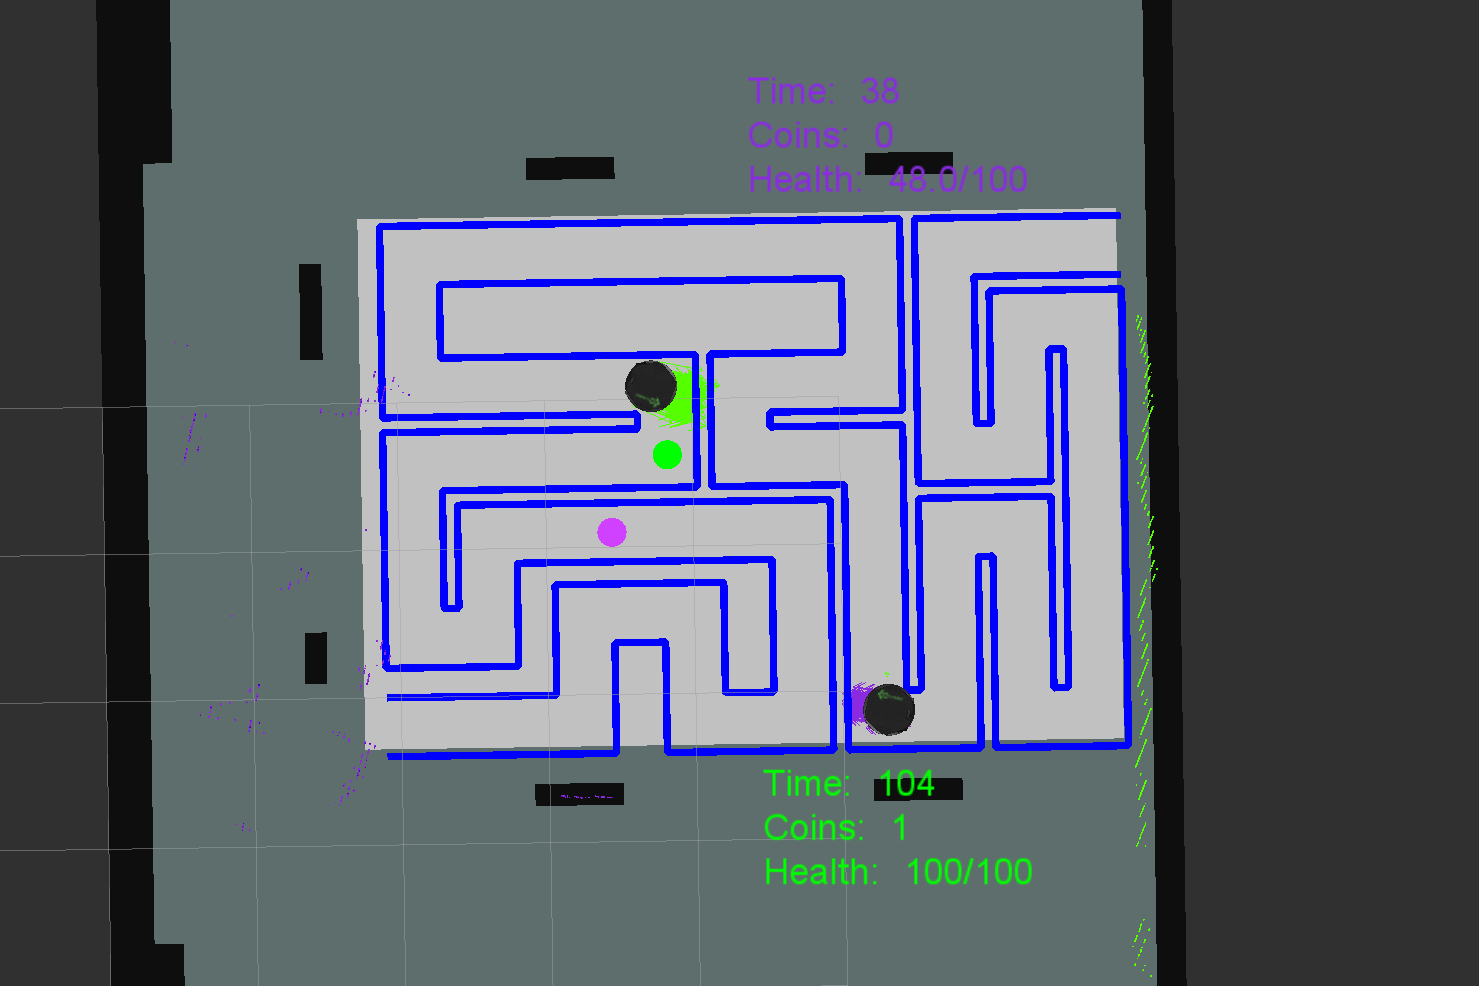
\includegraphics[width=.5\textwidth]{coin_game_rviz.png}
\caption{Maze map of the Coin Game experiment with coin goals.}
\label{fig:coin_map}
\end{figure}

The coin game is a very simple game. The human operator points the
mouse to a location the map. As the goal is random, the human operator
must now switch between robots frequently, in order to marshal the
various robots toward their coin goals. Research
\cite{olsen2003metrics} has shown that this switching time can affect
the effectiveness of a task performed by a human-robot team. Thus
the second experiment is more challenging in terms of cognitive
stress.  The task sets a two-minute timer for the human operator and
also sets a maximum 5 coin collection limitation. Either condition
satisfies the end of the game. Every time the robot collects a coin
the timer is shortened by 12 seconds to put more cognitive stress on
human operator.

In this instance, the robot has access only to what it can measure
about human behavior, in the form of the vector $H$.  It knows nothing
about what constitutes success in the Coin Game, as it is not even
able to sense the existence of coins.  However, it can still compute
$\hat{s} = g(H)$, and it can thus calculate an estimate of human
cognitive capacity and reliability.

In the coin game the human operator could interact with the robots using two interfaces; web browser (Fig.\ref{fig:web_interface_img}) and Rviz (Fig.\ref{fig:coin_map}). Among human operators ten people interacted with the robot remotely via web browser while playing the coin game. Whereas, ten other participated in the coin game being in the sane room where the game was staged via Rviz interface.
While using web interface, in order to compare the robot's estimate of cognitive capacity with
reality, test subjects were asked during the experiment to rate their
own cognitive stress levels at 12-second intervals using a Likert
scale. The human operators who participated using Rviz were given a physiological activity monitor\footnote{https://www.zephyranywhere.com/products/bioharness-3} to attach to their chest to monitor their heart rate, breathing rate, posture, ECG amplitudes and they were also being montitored by a human evaluator who rated and logged their cognitive stress level while they were playing the game. In other words human(coder) evaluator serves here as an subjective evaluator whreas the physiological metrics provides objective evaluation. Physiological metrics as objective evaluation along with subjective evaluation by the coder has been used and recommended in several works on human psycology\cite{Brookings1996361, Roscoe1992259}. We have found posture of human operator most likely correlates with subjective correlation with the code evaluation. One possible reason behind this is that posture is one of the visible observation that the coder can have while evaluating the operator. The coder rated stress level high when the operator tends to lean toward the screen of the computer when he or lean back on the chair. Other physiological metrics does not highly correlates with coder evaluation of stress level.

The coin game also had a autonomous assistant configuration where the robot starts to navigate the maze autonomously not knowing where the coin is. Robot can pick the coin if crossed over it.The autonomous mood was activated by the robot if it found the human operator to be untrustworthy; the stress level is higher than a threshold. The threshold that we have set for our experiment was 55\% based on the data that we have collected from the non autonomous or manual mood. If the ignorance time which is the duration while no commands were given to that particular robot was higher than a threshold the robot switched to autonomous mood as well. In autonomous mood robot assumes that the coin can show up anywhere in the maze thus moves towards the optimum way point from where it the expected distance from a coin is minimum. 
%We have set two scenarios in this experiment. The first scenario, is the single human operator one or more robots team. In this scenario only one human operator was allowed to assist the human-robot team. We have set a timer for the human operator as 2 minutes and also set maximum 5 coin collection limit. Either condition satisfies the end of the game. Every time the robot collects a coin the timer is shortened by 12 seconds to put more cognitive stress on human operator. In the second scenario, multiple one or more robots were teamed up with two human operators. The initial timer was set to 1 minute and a maximum of ten coins were allowed to collect. Either condition satisfied he end of the game.

\subsection{Coin Game Results}

Analysis of the results from the coin game experiment are in agreement
with the original hypothesis. In general, the robot correctly predicts
the cognitive load that its operator was under in every
scenario. These findings can be seen in Fig~\ref{fig:coder_eval_1_2}.
Here, the horizontal axis denotes model estimated cognitive stress over time. The vertical axis denotes coder evaluation cognitive load estimate. From our experiments we have found that the cognitive load estimate from the robots using our model correlates with the coder evaluated stress level by a factor $\rho=.205$ and $\rho=.25$ for coin game played with one and two robots respectively. Our experiment also captures that posture and breathing rate of human operator as objective metric for estimating cognitive stress level.We could not find any intersting pattern in other physiological objective metrics i.e. heart rate, ECG amplitude using our model and experimental setup. However, that does not mean that they do not capture cognitive stress level of human operator. A better model with more enriched $H$ vector of human behavior metric can certainly produce a better estimate that correlates more with those physiological metrics. But having a $H$ also means the robot can take more sophisticated input from human operators. Whereas in our case we have confined our experiment with simplistic robots.
It is critical for interpreting the information in \ref{fig:final-results} to note that while the robot's cognitive load evaluation and the scoring technique for quantifying
self-reported user stress both produce a result between zero and one
\textit{their magnitudes are not directly comparable}.Whenever cognitive stress occurs or changes, the robot is able to recognize this increase for most cases in the
tested scenarios, and the robot's evaluation agrees with self-reported
user stress.

\begin{figure}  
\centering
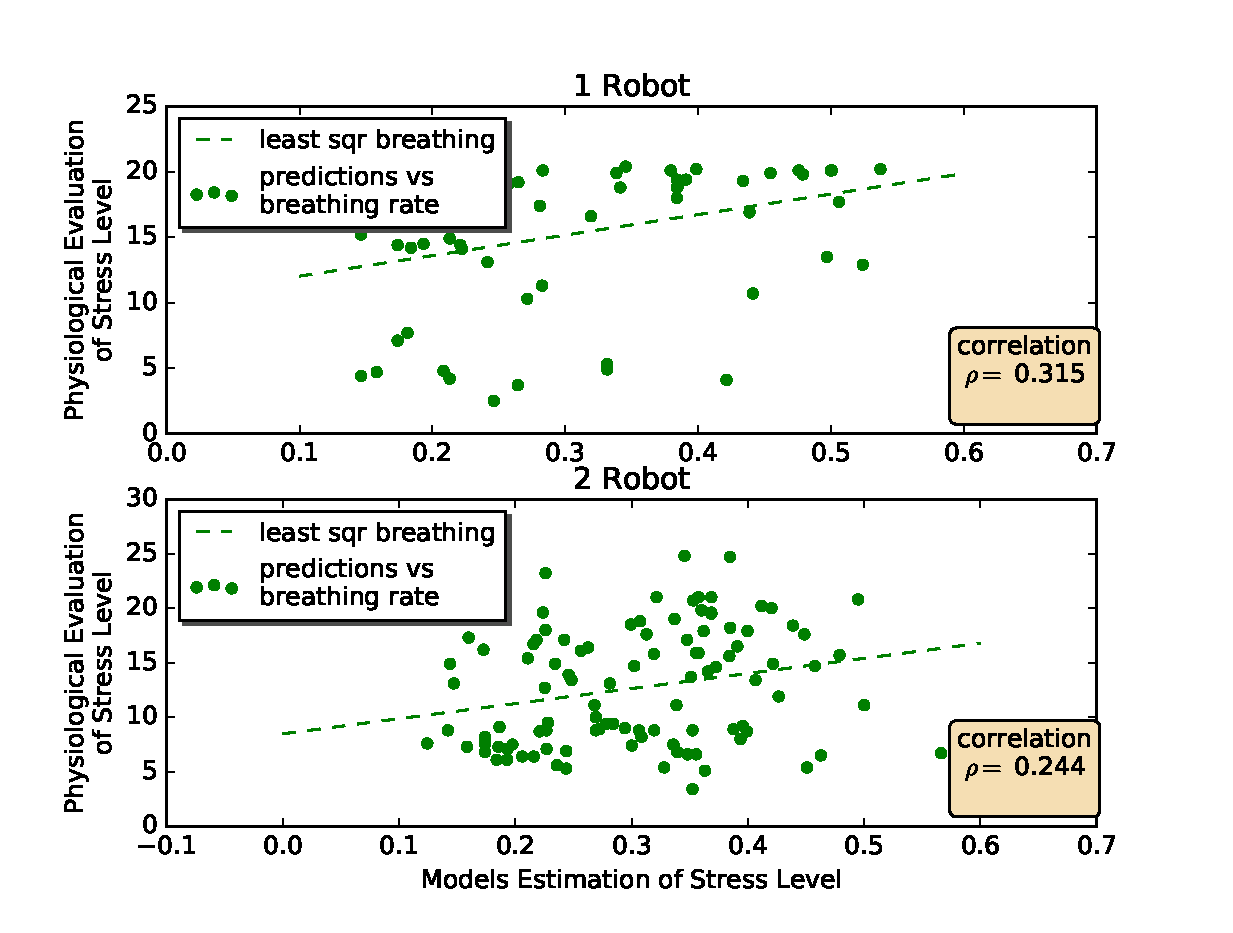
\includegraphics[width=.5\textwidth]{prediction_vs_b_p_2.eps}
\caption{Models predicted stress level vs Physiological metrics in coin game experiment.}
\label{fig:pred_phy}
\end{figure}

Most important contribution of our model can has been demonstrated from the perspective of task success. The task success of the coin game is measured in term of number of coins collected withing given time. Our experiment shows that by switching to autonomous mood on detection of high stress level of human operator can significantly improve the task success Tab.\ref{tab:task_success}. Table \ref{tab:task_success} shows that dealing with more number of robots requires high cognitive labor for the human operator causing less winning rate and more time requirement. However, when we provide autonomous assistance on detection of high stress level using our learned model which was learned from another task, it improves overall task success.In the context of this paper, it also supports the original hypothesis: robots can are able to reliably assess the cognitive strain their human partners are under, even in contexts where the actual tasks they are being asked to perform are opaque to the robot.

\begin{figure}
\centering
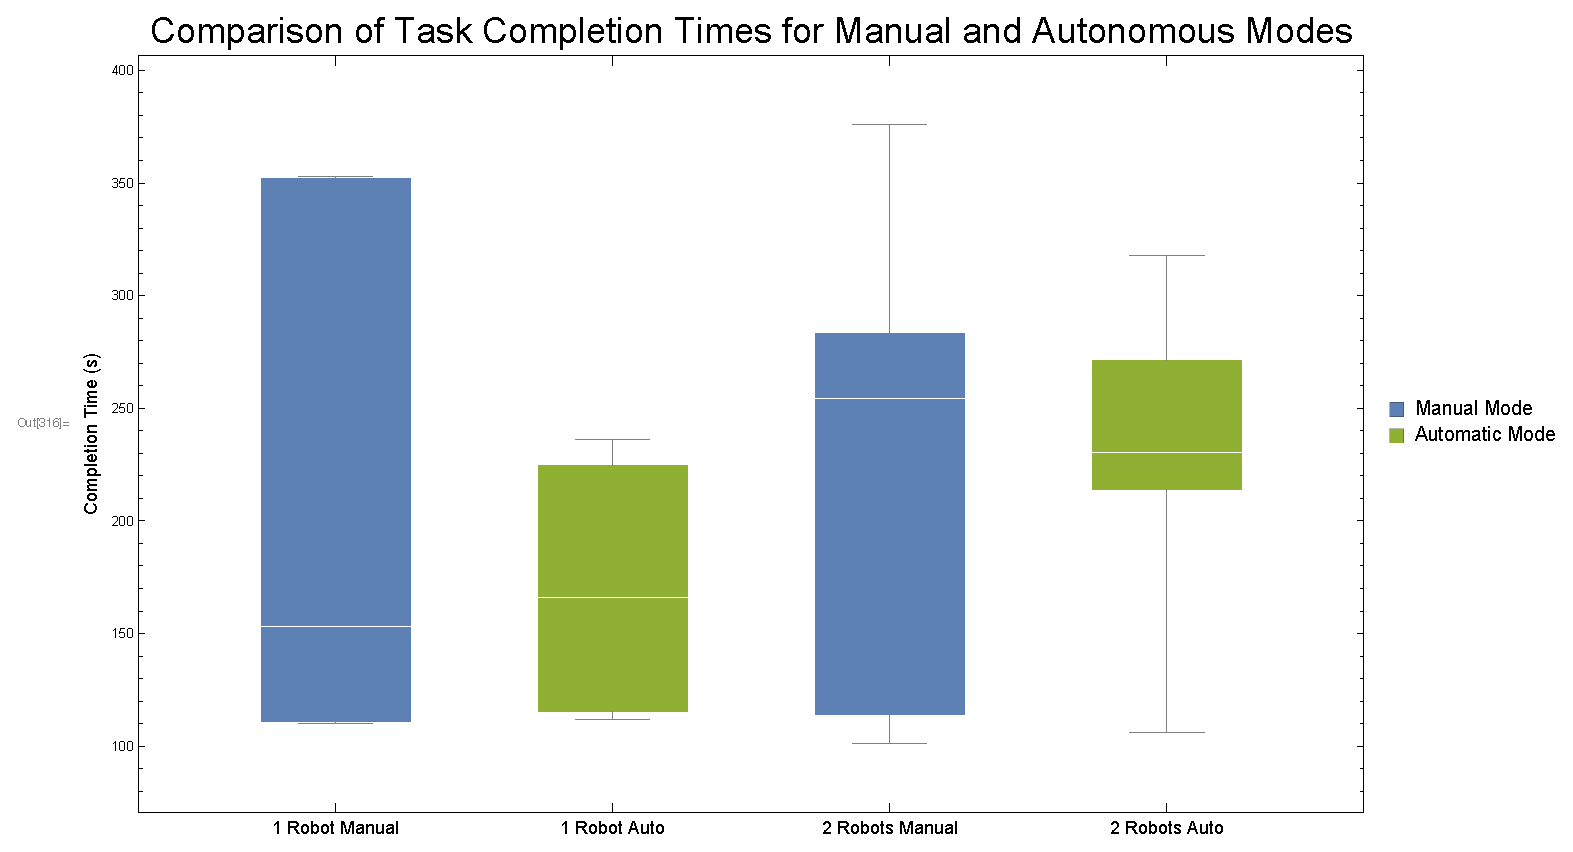
\includegraphics[width=.5\textwidth]{BoxWiskerTimesCompMaualVsAuto.eps}
\caption{"Test"}
\label{fig:BoxWiskersTimeComp}
\end{figure}

% Please add the following required packages to your document preamble:
% \usepackage{booktabs}
\begin{table}[]
\centering
\caption{Task success comparisons between autonomous assistance mood and manual mood. Autonomous assistance was activated on detection of high stress level predicted by our model.}
\label{tab:task_success}
\begin{tabular}{@{}|c|c|c|c|c|@{}}
\toprule
Game Mode                                                                                  & \multicolumn{2}{c|}{Manual} & \multicolumn{2}{c|}{\begin{tabular}[c]{@{}c@{}}Autonoumous \\ Assitance on high\\ Stress level\end{tabular}} \\ \midrule
\begin{tabular}[c]{@{}c@{}}Number of\\ Robots\\ Participated\end{tabular}               & one          & two          & one                                                   & two                                                  \\ \midrule
\begin{tabular}[c]{@{}c@{}}Number of Failure/\\ Total Number\\ of Game Played\end{tabular} & 2/12         & 5/15         & 0/10                                                  & 1/10                                                 \\ \midrule
\begin{tabular}[c]{@{}c@{}}Average time\\ per game\\ (in sec.)\end{tabular}                & 329          & 345          & 170                                                   & 233                                                  \\ \bottomrule
\end{tabular}
\end{table}

%Six people who participated in first experiment also participated in
%the second experiment. We have found that the learned model of
%classifier was able to understand good and bad assistance very
%efficiently. We did not allow the robot to change its behavior based
%on the trustworthiness; it is just keeping a log of which of the
%assistance came from the human operator were trustworthy and which
%were not. While running the second experiment we manually kept a log
%to indicate which particular human assistance were seemed to be
%trustworthy in the naked eye. After the experiment we collected the
%log from the robot and then compared with our human judged
%interpretation of trustworthiness. We have found that the 95\% and
%97\% of robots prediction matches with the two human
%interpretations. This is a very promising result to support our
%hypothesis in Eq.~\ref{eq:trust_norm}. The result also showed decrease
%in trustworthiness as the complexity of the task increases. The result
%on matching classification on different level of complexities are
%shown in the following Fig\ref{fig:final-results}:
%\begin{figure}  
%\centering
%%
\includegraphics[width=.25\textwidth]{final-legend.eps}
%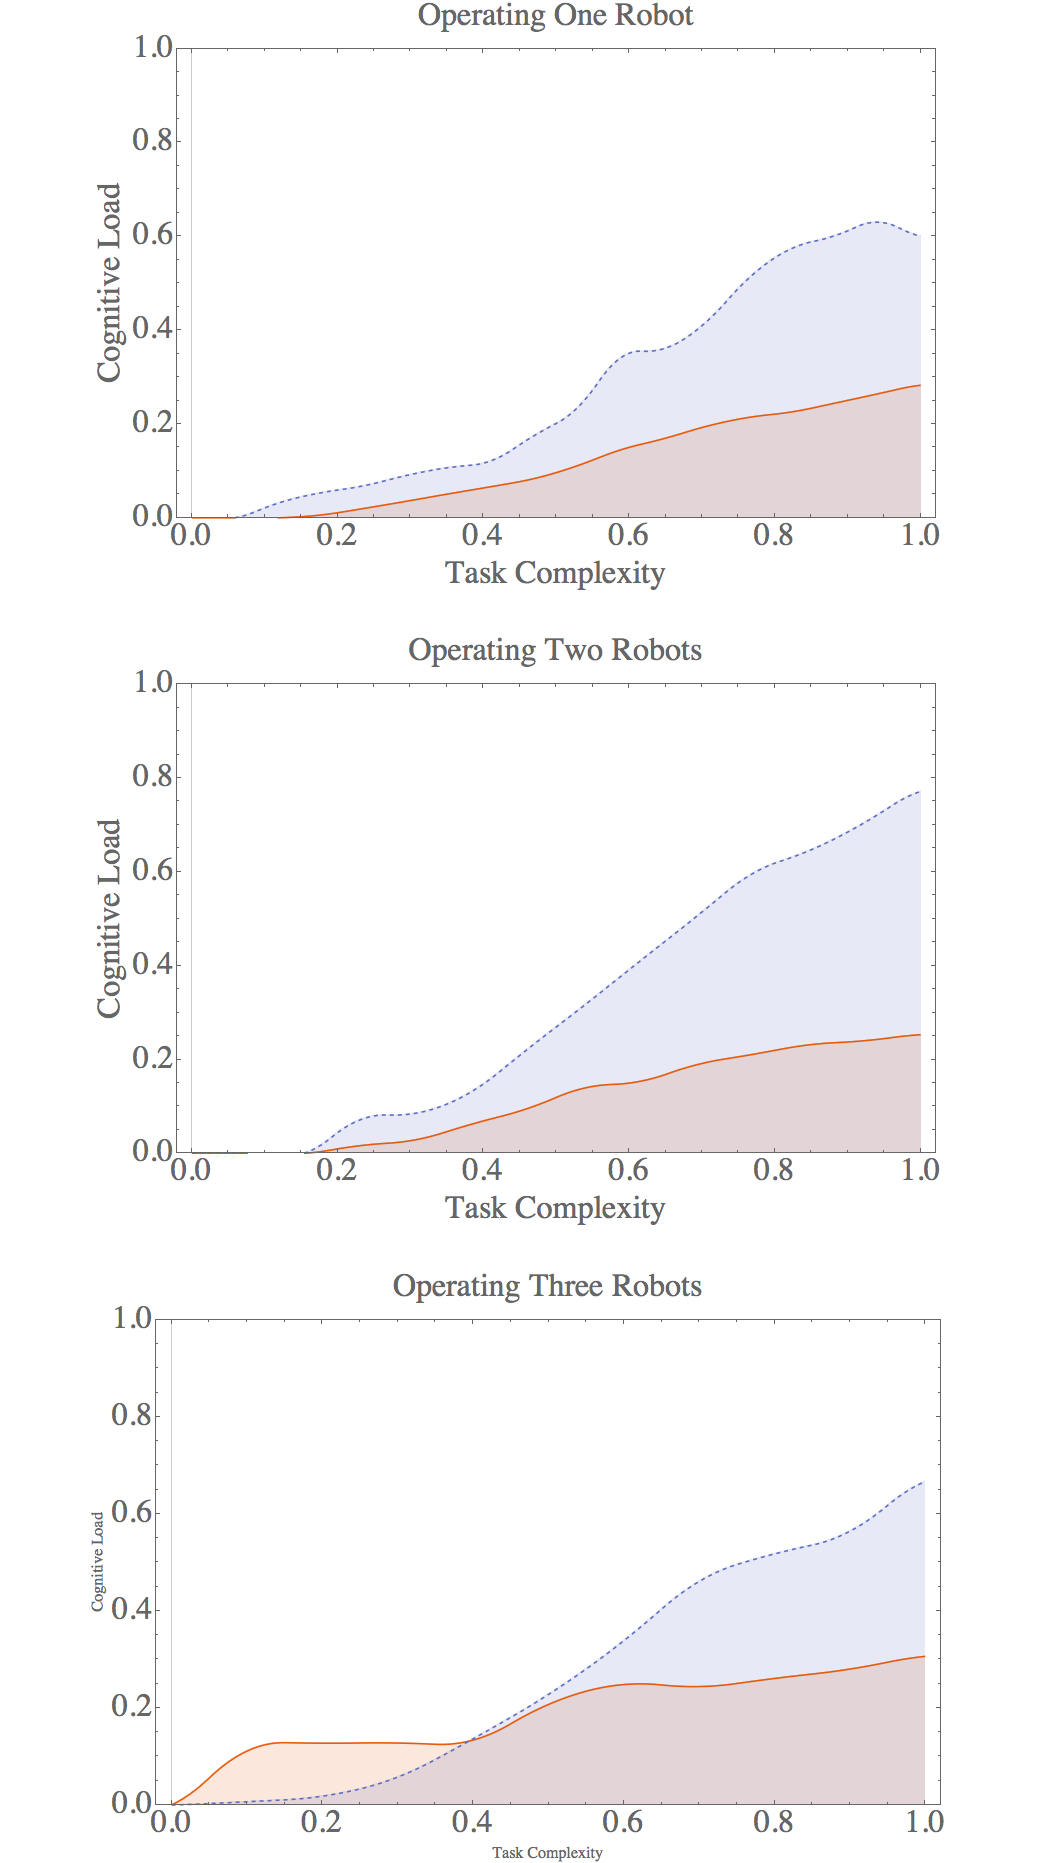
\includegraphics[width=.4\textwidth]{final-results.png}
%\caption{Cognitive load of human operators in Coin Game experiments with differing numbers of robots and steadily increasing task complexity.  Blue represents subject self-reporting, orange the robot's estimate of $\hat{s}$.}
%\label{fig:final-results}
%\end{figure}

\begin{figure}  
\centering
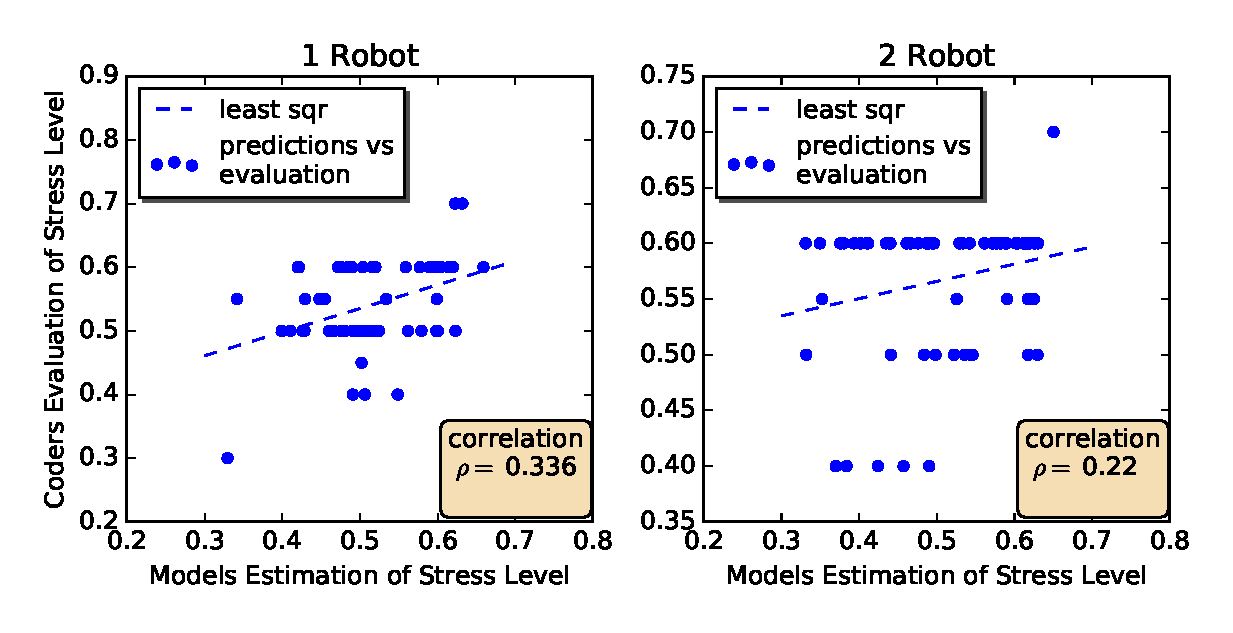
\includegraphics[width=.5\textwidth]{coder_eval_1_2.eps}
\caption{Cognitive load of human operators in Coin Game experiments with differing numbers of robots and steadily increasing task complexity. The robots' predictions fairly correlates with the coder evaluation of cognitive load estimate.}
\label{fig:coder_eval_1_2}
\end{figure}


\section{Conclusions}

The field of human-robot interaction began by investigating how robots
can be designed so that they are comfortable, predictable and
understandable to their human partners.  Our work investigates an
aspect of the other side of that equation: what can robots understand
about us?  Robots that are capable of understanding the stress or
strain their operator is experiencing are vital to safe and efficient
teamwork in complex scenarios where the proper level of autonomy and
interaction is fluid.  Vital communication cues are embedded in the
way we behave in particular circumstances, and these implicit
indicators do not have to be lost on our robots.  Our work's
contribution is to demonstrate a quantitative, learnable,
generalizable model that allows a robot to determine that a user is
behaving in an untrustworthy fashion, even when the robot cannot
independently assess the instructions it is being given.  Another
important finding is that the threshold beyond which cognitive stress
produces untrustworthy human assistance may vary from task to task.
Nevertheless, general metrics can transfer from problem to problem and
still produce meaningful evaluations.  In the future, we plan to
extend this research into complex heterogeneous teams of humans and
robots performing real-world tasks.

Every day humans interact with more and more technologies that require
us to decide whether or not to trust them; robots should be making
similar determinations about us.

%Our research has a profound implication on the way used to look into
%human robot team. One vital contribution of this paper is that it
%shows that trustworthiness of human operator in human-robot team can
%be quantified and learned using useful metrics. We can define it by
%the term transfer effectiveness of human operator. Besides, defining
%this novice terminology we have also achieved significant evidence to
%show transfer effectiveness is possible across multiple problem
%domain. We have done two experiments on human-robot team to assess
%cognitive capacity of human assistance. For our a particular problem
%of maze game, metrics like our disparity, arrival time delay and
%damage considered as vital metrics in determining the
%trustworthiness. We have shown that the learned model also implies on
%Coin Game problem which our second experiment. Although, built on
%similar set-up, the second experiment was different in many ways from
%the first. We showed that, although they are different the
%trustworthiness classifier model can be transferred to this new domain
%of problem effectively. From this experimental result we try to say
%that for if several human-robot team problems have metrics those have
%common implications, may help us to learn the nature of of human
%assistance cognitive behaviour for those problems. It may also help us
%to infer the human cognitive stress limitation in another problem. In
%other words, our research showed that cognitive capacity of human
%assistant is transferable.


\section{Acknowledgments}
Support for this work was provided by a National Science Foundation
RII Track-2 FEC award (Unmanned Aircraft System for Atmospheric
Physics).

%We would like to thank Robotic Cognition Laboratory of Computer Science Department of Oklahoma State University for facilitating this project. We would also like to thank all the people who participated in the project as human operator voluntarily.

\bibliographystyle{abbrv}
%\bibliographystyle{acmlarge}
\bibliography{sigproc-2}

\end{document}
